\section{Leptons}
\label{chp:obj:lep}

The reconstruction and identification of electrons and muons is discussed. In this dissertation $\tau$-leptons are not explicitly used, thus $\tau$-lepton reconstruction techniques are not described. Although no attempt is made to identify $\tau$-leptons, they would be identified either as isolated electrons or muons, or as (narrow) jets according to their decay.


\subsection{Electrons}
\label{chp:obj:sec:ele}
The reconstruction of electrons in the central region of the ATLAS detector ($|\eta| < 2.47$) starts from energy deposit (clusters) in the EM calorimeter, which are then associated to reconstructed tracks in the ID. A sliding-window algorithm \cite{ATLAS-CONF-2016-024} is used to search for electron clusters. Seed clusters are established as longitudinal towers consisting of $3\times5$ calorimeter segments ($\Delta \eta \times \Delta \phi = 0.025 \times 0.025$, the granularity of the calorimeter middle layer)  with transverse energy $E_{\rm T}> 2.5 \, \gev$. Electron candidates are formed as seed clusters matched to at least one ID track. The standard pattern recognition for track reconstruction uses the pion hypothesis for energy loss at material surfaces. A modified pattern-recognition algorithm for the electron hypothesis allows at most $30\%$ energy loss at each material surface to account for possible bremsstrahlung. Thus, track candidates are fitted either with the pion hypothesis or the electron hypothesis. Tracks, extrapolated in the calorimeter middle layer, are then matched with relaxed criteria to EM clusters. Matched tracks are refitted with stricter conditions to build electron candidates. The track associated with the electron has to be compatible with the hard-scatter PV in order to reduce the background from conversions and secondary particles. The following requirements are made: $|d_{0}|/\sigma_{d_{0}}< 5$ and $|z_{0} \sin \theta| < 0.5$ mm, where $d_{0}$, $z_{0}$ and $\theta$ are defined in section \ref{chp:obj:trk}. The electron cluster is then rebuilt using $3\times7$ ($5\times5$) longitudinal towers of cells in the barrel (endcaps) of the EM calorimeter. The energy of the clusters is calibrated to the original electron energy using multivariate techniques \cite{ATL-PHYS-PUB-2016-015} based on simulated MC samples.
The calibrated cluster energy is determined as a sum of the measured energy deposit in the cluster and the estimated energy deposits in the material in front of the EM calorimeter, in the neighbouring EM segments (lateral leakage) and beyond the EM calorimeter (longitudinal leakage). The momentum of the matched track is also used in the calculation. The $\eta$ and $\phi$ directions of an electron are those of the corresponding track, unless the track contains only TRT hits, in which case the $\eta$ is determined from the cluster pointing ($\eta_{\rm cl}$) due to the insufficient resolution of the TRT.

\bfig[t!]
\centering
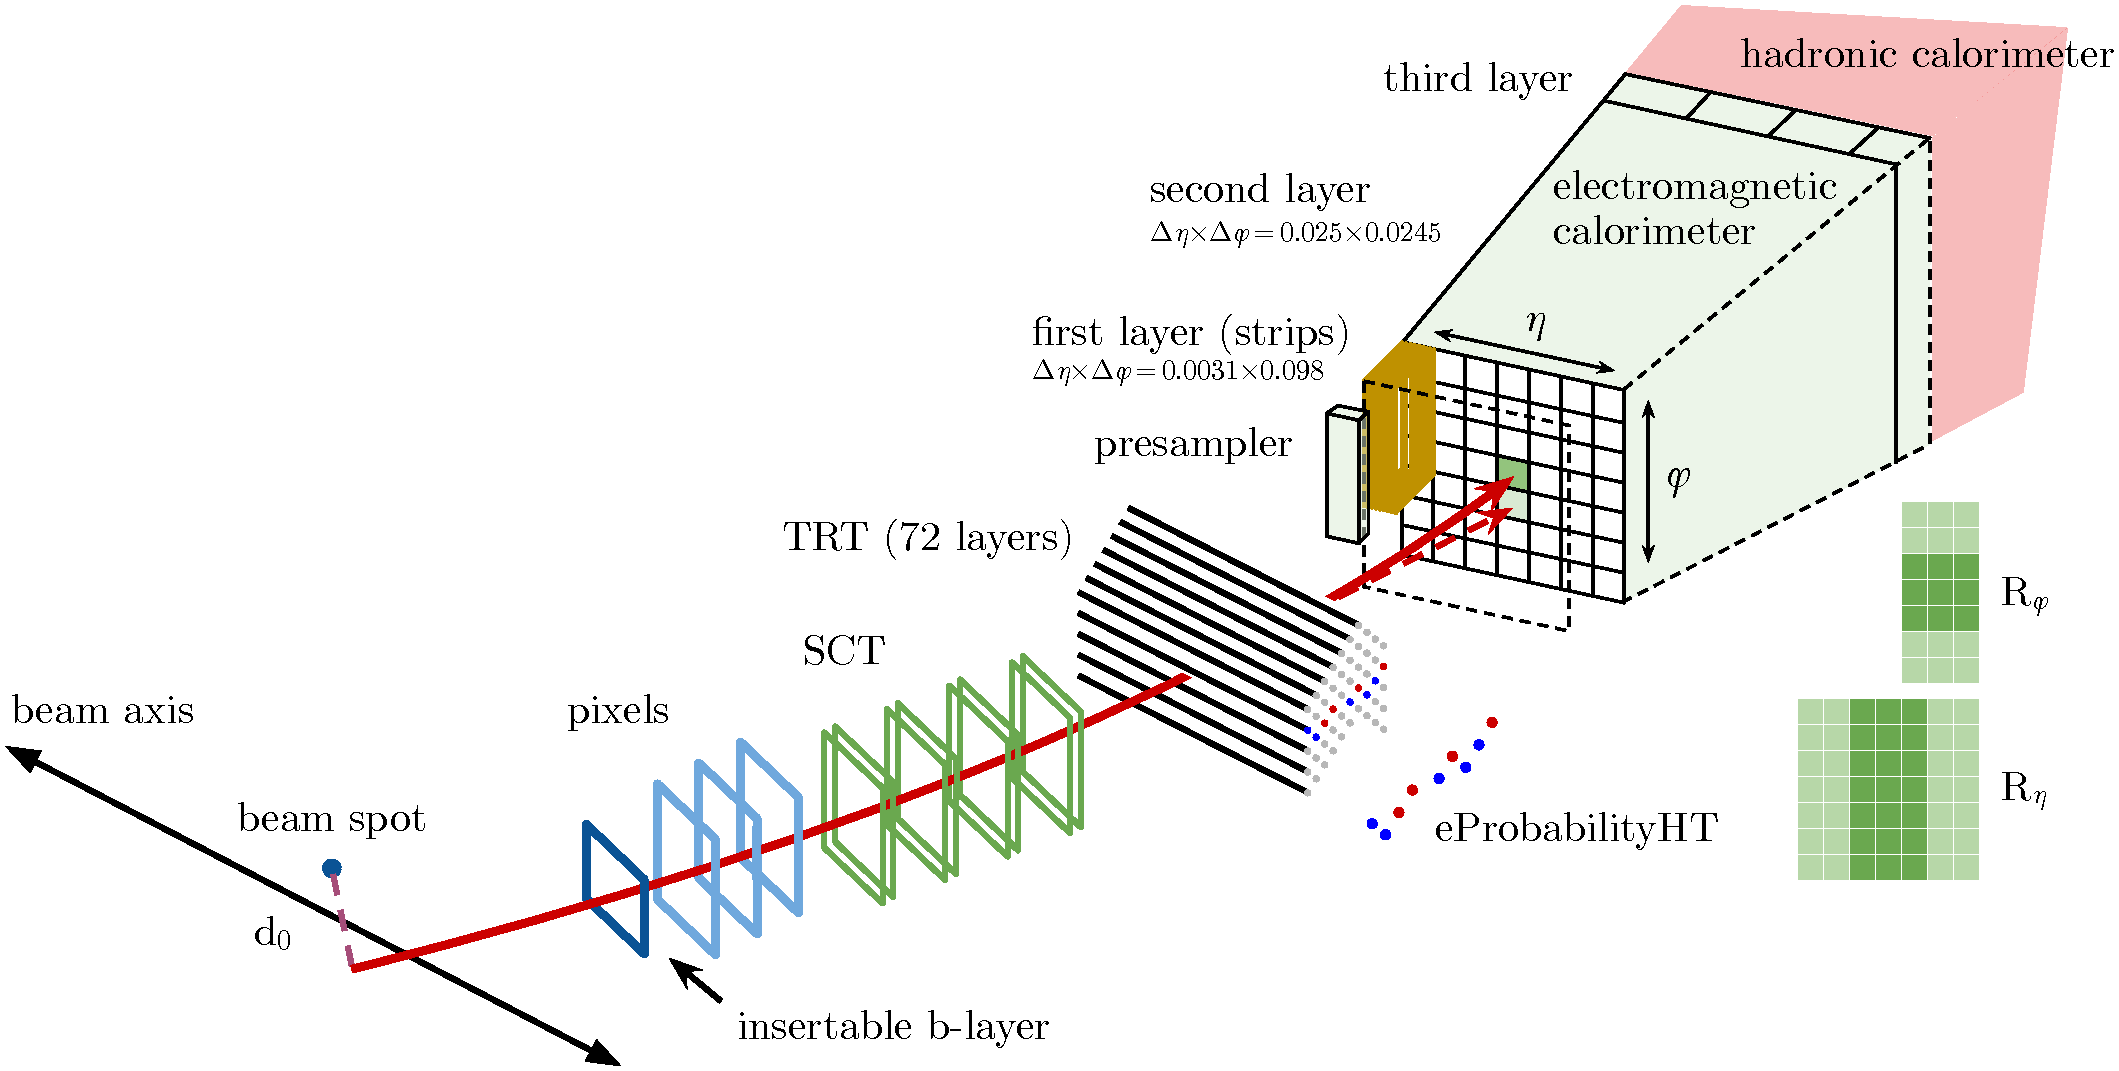
\includegraphics[width=0.8\textwidth]{figures/Objects/eleillustration.png}
\captionsetup{width=0.85\textwidth}  \caption{\small Illustration of the electron reconstruction and identification.}
\label{sec:obj:fig:elerec}
\efig


Electron identification algorithms \cite{ATLAS-CONF-2016-024} use quantities related to the electron cluster and track measurements including calorimeter shower shapes, information from the TRT, track-cluster matching-related quantities, track properties, and variables measuring bremsstrahlung effects used to distinguish electrons from background mimicking them (e.g. hadronic jets or converted photons). The shower development is narrower for electrons than for hadrons, and the hadronic leakage is smaller. Track-quality requirements reduce the impact of accidental track association with photons, energetic $\pi^{0}$ or $\eta$ mesons with electromagnetic decays reconstructed as a single energy cluster. The baseline identification algorithm exploits several properties of the electron candidate, combined using a likelihood-based (LH) method.\footnote{The LH method uses the signal and background probability density functions (PDFs) of the discriminating variables. Based on these PDFs, an overall probability, defined as the product of the individual PDFs, is calculated for the object to be signal or background.} The list of the discriminating variables used in the electron LH can be found in table \ref{tab:obj:lep:elevar}.
\begin{table}\footnotesize
\begin{center}
\begin{tabular}{|c|c|c|}
  \hline \hline
   Type & Name & Description \\
  \hline
 Hadronic leakage & $R_{\rm had1}$ &  Ratio of $\eT$ in the first layer of the hadronic calorimeter to $\eT$ \\
 & &  of the EM cluster (used over the range $|\eta|< 0.8$ or $|\eta|> 1.7$)\\
 \cline{2-3}
 & $R_{\rm had}$ &  Ratio of $\eT$ in the hadronic calorimeter to $\eT$\\
 & &  of the EM cluster (used over the range $0.8<|\eta|< 1.7$)\\
 \hline
 Back layer of & $f_{3}$ & Ratio of the energy in the back layer to the total energy\\
 EM calorimeter & & in the EM accordion calorimeter (used <100 \gev )\\
 \hline
 Middle layer of & $w_{\eta2}$ &Lateral shower width, $\sqrt{(\sum E_{i}\eta_{i}^{2})/(\sum E_{i})-((\sum E_{i}\eta_{i})/(\sum E_{i}))^{2}}$,\\
 EM calorimeter & & where $E_{i}$ is the energy and $\eta_{i}$ is the pseudorapidity of cell $i$ and\\
 & &  the sum is calculated within a windows of $3\times 5$ cells\\
  \cline{2-3}
  & $R_{\Phi}$ & Ratio of the energy in $3\times3$ cells over the energy in $3\times7$ cells\\
  & & centered at the electron cluster position\\
   \cline{2-3}
   & $R_{\eta}$ & Ratio of the energy in $3\times7$ cells over the energy in $7\times7$ cells\\
   & & centered at the electron cluster position\\
   \hline
   Strip layer of& $w_{\rm stot}$ & Shower width, $\sqrt{(\sum E_{i}(i-i_{\rm max})^{2})/(\sum E_{i})}$, where $i$ runs over all\\
   EM calorimeter& & strips in a window of $\Delta \eta \times \Delta \phi \approx 0.0625 \times 0.02$, corresponding typically \\
   & &  to 20 strips in $\eta$, and $i_{\rm max}$ is the index of the highest-energy strip\\
   \cline{2-3}
   &$E_{\rm ratio}$&Ratio of the energy difference between the largest and second\\
   && largest energy deposits in the cluster over the sum of these energies\\
   \cline{2-3}
   &$f_{1}$&Ratio of the energy in the strip layer to the total energy\\
   &&in the EM accordion calorimeter\\
   \hline
   Track conditions & $n_{\rm Blayer}$ & Number of hits in the innermost pixel layer (IBL)\\
   \cline{2-3}
   & $n_{\rm Pixel}$ & Number of hits in the pixel detector\\
   \cline{2-3}
   & $n_{\rm Si}$ & Number of total hits in the pixel and SCT detectors\\
   \cline{2-3}
   & $d_{0}$ & Transverse impact parameter with respect to the beam-line\\
   \cline{2-3}
   &$d_{0}/\sigma_{d_{0}}$& Significance of transverse impact parameter defined as\\
   & & the ratio of $d_{0}$ and its uncertainty\\
   \cline{2-3}
   &$\Delta p /p$&Momentum lost by the track between the perigee and the last\\
   &&measurement point divided by the original momentum\\
   \hline
   TRT& eProbabilityHT& Likelihood probability based on transition radiation in the TRT\\
   \hline
   Track-cluster&$\Delta \eta_{1}$&$\Delta \eta$ between the cluster position in the strip layer\\
   matching&&and the extrapolated track\\
    \cline{2-3}
    &$\Delta \phi_{2}$&$\Delta \phi$ between the cluster position in the middle layer and\\
    && the track extrapolated from the perigee\\
     \cline{2-3}
     &$\Delta \phi_{\rm res}$&Defined as $\Delta \phi_{2}$, but the track momentum\\
     && is rescaled to the cluster energy before extrapolating the track from \\
     &&the perigee to the middle layer of the calorimeter\\
     \cline{2-3}
     & E/p& Ratio of the cluster energy to the track momentum\\     
 \hline\hline
  

\end{tabular}
\captionsetup{width=0.85\textwidth}  \caption{\small Discriminating variables used in the electron LH.}
\label{tab:obj:lep:elevar}
\end{center}
\end{table}
\noindent Several changes to the input variables have been introduced for Run 2. The number of hits in the innermost pixel layer discriminates electrons against converted photons and, with the installation of the IBL, this variable was redefined. Furthermore, a LH based on the TRT high-threshold hits (eProbabilityHT) is introduced to compensate for the lower transition radiation absorption probability, due to the change of the gas (Ar). \par
Three operating points for electron identification, with increasing background rejection, are defined: {\sl Loose}, {\sl Medium} and {\sl Tight}. Operating points are defined such that the samples selected by them are subsets of one another (e.g. electrons satisfying the {\sl Medium} criteria also satisfy the {\sl Loose} criteria). Since the distributions of electron shower shapes depend on the amount of material traversed by electrons and on the number of pileup collisions per bunch crossing, the ID operating points were optimised in several bins of $|\eta|$ and $\eT$ and as a function of the number of primary vertices, in order to ensure efficient identification at high pileup. The electron identification efficiency is measured in $Z\to e^{+}e^{-}$ events in data and MC using the tag-and-probe method, as illustrated in figure \ref{sec:obj:fig:eleeff}.

\begin{figure}[h!]
\begin{subfigure}{0.5\textwidth}
  \centering
  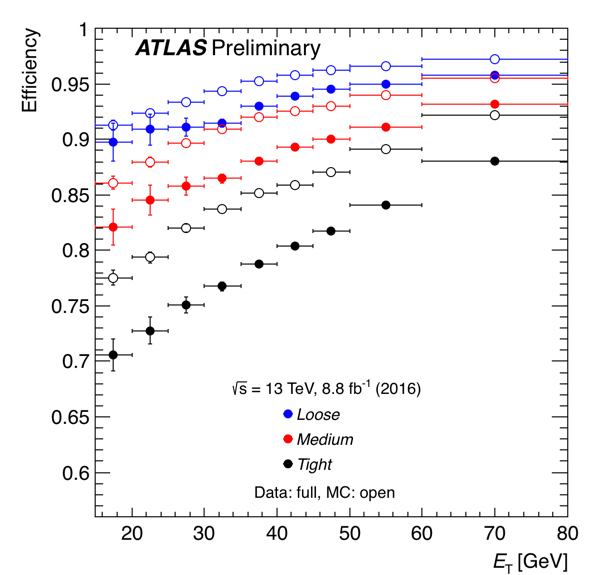
\includegraphics[width=0.9\textwidth]{figures/Objects/effeleet.png}
  \caption{}
  \label{sec:obj:fig:eleeffet}
\end{subfigure}
\begin{subfigure}{0.5\textwidth}
  \centering
  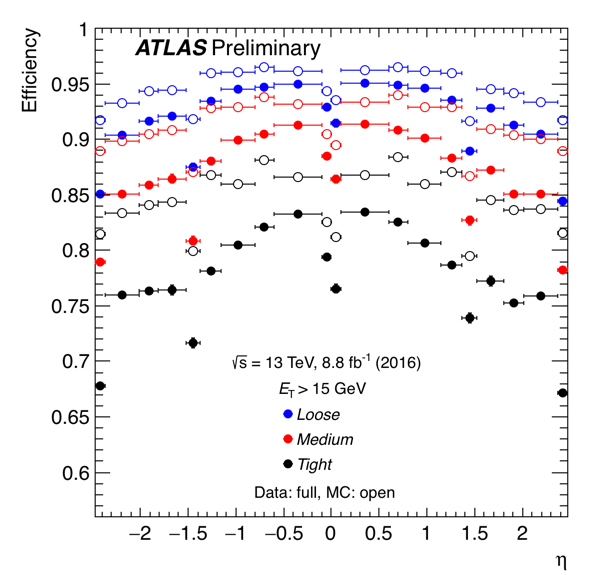
\includegraphics[width=0.9\textwidth]{figures/Objects/eleeffeta.png}
  \caption{}
  \label{sec:obj:fig:eleeffeta}
\end{subfigure}
\begin{center}
\begin{subfigure}{0.5\textwidth}
  \centering
  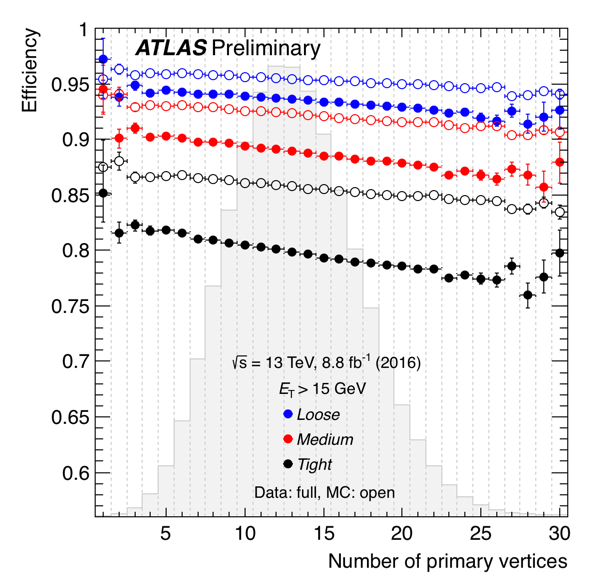
\includegraphics[width=0.9\textwidth]{figures/Objects/eleeffnpv.png}
  \caption{}
  \label{sec:obj:fig:eleeffnpv}
\end{subfigure}
\end{center}
\captionsetup{width=0.85\textwidth}  \caption{\small Electron identification efficiencies for the different operating points obtained using the tag-and-probe method in $Z \to e^+e^-$ events, as a function of (a) transverse energy $\eT$, (b) pseudorapidity $\eta$ and (c) number of reconstructed primary vertices. From reference \cite{ATLAS-CONF-2016-024}.}
\label{sec:obj:fig:eleeff}
\end{figure}

To further disentangle prompt electrons from electrons or photons produced in hadron decays, an additional requirements on the total transverse momentum within a cone around the electron direction are imposed. The selection exploits both track-based and calorimeter-based isolation. The track isolation variable $\pt^{\rm varcone0.2}$ is the sum of the transverse momenta of all the tracks within a cone of size $\Delta R = \min(0.2,10\,\gev/\eT)$ around the electron direction. Only tracks with $\pt > 1 \,\gev$ and compatible with originating from the hard-scatter PV are considered, with the exception of the track used to build the electron candidate. The  cone size is chosen to be $\pt$-dependent to improve performance for electrons produced in the decay of particles with large transverse momentum. The calorimetric isolation variable $\eT^{\rm cone0.2}$ represents the sum of the transverse energy of the calorimetric cells in a cone of size $\Delta R=0.2$ around the electron, after subtraction of the energy deposits associated with the electron itself and pileup contributions. A variety of operating points are provided with different requirements on $\eT^{\rm cone0.2}/\eT$ and $\pt^{\rm varcone0.2}/\pt$. The isolation efficiency corresponding to these operating points can be either constant or a function of $\eT$. The isolation efficiency for the various operating points estimated for electrons from simulated $Z\to e^{+}e^{-}$ events is summarised in table \ref{tab:obj:lep:eleiso}. 

\begin{table}\footnotesize
\begin{center}
\begin{tabular}{|c|c|c|c|}
  \hline \hline
   Electron isolation OP & Calorimeter isolation efficiency & Track isolation efficiency & Total efficiency \\
  \hline
  {\sl LooseTrackOnly} & - & 99$\%$ &99$\%$\\
 {\sl Loose} & 99$\%$& 99$\%$ &$\sim98\%$\\
   {\sl Tight} & 96$\%$& 99$\%$ &$\sim95\%$\\
   {\sl Gradient}&$0.1143\%\times \eT + 92.14\%$& $0.1143\%\times \eT + 92.14\%$&90/99$\%$ at $E_{\rm T}=$25/60 \gev\\
{\sl GradientLoose}&$0.057\%\times \eT + 95.57\%$& $0.057\%\times \eT + 95.57\%$&95/99$\%$ at $E_{\rm T}=$25/60 \gev\\
 \hline \hline
\end{tabular}
\captionsetup{width=0.85\textwidth} \caption{\small Electron isolation efficiency operating points (OP).}
\label{tab:obj:lep:eleiso}
\end{center}
\end{table}


Reconstruction, identification, isolation, and trigger efficiencies are the different components of the total efficiency $\epsilon_{\rm total}$ to find and select an electron in the ATLAS detector:

\be
\epsilon_{\rm total}=\epsilon_{\rm reconstruction}\times \epsilon_{\rm identification}\times \epsilon_{\rm isolation}\times \epsilon_{\rm trigger},
\ee

\noindent with the various components measured relative to the previous requirement. To measure those efficiencies the tag-and-probe method is used.
The method employs events containing well-known resonance decays to electrons ($Z\to e^{+}e^{-}$ and $J/\Psi\to e^{+}e^{-}$) with strict selection criteria on the event selection and on one of the electron (``tag''). The ``probe'' electron is used for the measurement of the reconstruction, identification, isolation
and trigger efficiencies, after accounting for the residual background contamination. The low-$E_T$ range (from 7 to 20 \gev) is covered by $J/\Psi\to e^{+}e^{-}$ events, while $Z\to e^{+}e^{-}$ events are used for measurements above 15 \gev. The efficiencies are estimated both in data and in simulation and their ratio is used as a scale factor to correct the simulation. These scale factors, derived as a function of electron $E_T$ and $\eta$, typically deviate from unity by only a few percent. The combined uncertainties on the reconstruction, identification, isolation and trigger requirement scale factors are at the level of few percent at low $E_T$ and below 1$\%$ at high $E_T$.\par
The electron energy scale has been measured in data using $Z\to e^{+}e^{-}$ event. Correction factors as a function of the electron $\eta$ are derived to match the known value of the $Z$-boson mass. The total uncertainty on the electron in-situ calibration is < 1$\%$ in the central region \cite{ATLAS-CONF-2016-024}. The main way to probe the electron energy resolution is provided by the study of the $Z$ resonance width. It is found that the resolution in data is slightly worse than that in simulation, and appropriate corrections are derived and applied to the simulation to match the data.\par
The analyses presented in this dissertation use the {\sl Tight} electron definition since it requires the largest possible rejection of misidentified electrons. Electrons are required to be central ($|\eta|$ < 2.47) and to be outside the transition region between the barrel and end-cap EM calorimeter ($1.37 <|\eta| < 1.52$), since this region shows worse reconstruction and energy resolution performances. Finally, electron isolation (\emph{Gradient} OP) is required to reject electrons from semileptonic hadron decays. A different electron definition, with looser selection criteria, is also be used to estimate the contribution of multijet events where a jet is reconstructed as an electron. This looser definition uses \emph{Medium} as identification criteria and no isolation requirement. The use of this looser electron set will be described in detail in section \ref{chp:sec:sigbkg:qcd}.


\subsection{Muons}
\label{chp:obj:sec:muon}
Muons are reconstructed using four different strategies \cite{Aad:2016jkr}, depending on which subdetectors are used in the reconstruction. Muons used in this dissertation are \emph{combined muons}, which exploit measurements from the ID and the MS. A pattern recognition algorithm forms segments in the MS starting from hits in the different subsystems. Muon track candidates in the MS are seeded by segments in the middle layers of the MS. The fitting procedure uses a combinatorial search to combine segments in the track candidate, taking into account the muon energy loss in the calorimeter. Once track candidates are built, an overlap removal procedure is applied to remove shared segments and the track is refitted with a stricter selection criteria. For combined muons, a global fit of ID and MS tracks is performed. Most muons are reconstructed following an outside-in algorithm, in which the muons are first reconstructed in the MS and then extrapolated inward and matched to an ID track. An inside-out combined reconstruction is used as a complementary approach. In Run 2, muon reconstruction algorithms have been improved providing a better background rejection in the pattern recognition and an improved calculation of the energy loss in the calorimeter \cite{Aad:2016jkr}.\par
Muon  identification  is performed  by  applying  quality  requirements  that  suppress  background,  mainly from pion and kaon decays, while selecting prompt muons with high efficiency and ensuring a robust momentum measurement. The variables used in the muon identification are listed below:

\bi
\ib $q/p$ significance, defined as the absolute value of the difference between the ratio of the charge and momentum of the muons measured in the ID and MS, divided by the sum in quadrature of the corresponding uncertainties;
\ib $\rho^{\prime}$, defined as the absolute value of the difference between the transverse momentum measurements in the ID and MS, divided by the $\pt$ of the combined track;
\ib normalised $\chi^{2}$ of the combined track fit;
\ib $\ge 1$ pixel hit;
\ib $\ge 5$ SCT hits;
\ib $<3$ Pixel or SCT holes;\footnote{A hole is defined as an active sensor traversed by the track but containing no hits.}
\ib at least 10$\%$ of the TRT hits originally assigned to the track are included in the final fit (in the $0.1< |\eta| <1.9$ range).
\ei

Four operating points for muon identification are defined: {\sl Loose}, {\sl Medium}, {\sl Tight} and {\sl High-$\pt$}. In this dissertation {\sl Medium} muons are used. The {\sl Medium} the identification criteria provides the default selection for muons in ATLAS, minimizing the systematic uncertainties associated with muon reconstruction and calibration. {\sl Medium} identification applies the following additional requirements on the muon:

\bi
\ib $\ge 3$ hits in at least two MDT layers except for tracks in the $|\eta|$ < 0.1 region, where tracks with at least one MDT layer but no more than one MDT hole layer are allowed;
\ib $q/p$ significance < 7.
\ei

Similarly to electrons, to further disentangle prompt muons from heavy-flavour hadron semileptonic decays, additional requirements on the total transverse energy and momentum within the corresponding cones around the muon direction are imposed. The selection exploits both track-based and calorimeter-based isolation. The track isolation variable $\pt^{\rm varcone30}$ is the sum of the transverse momenta of the tracks with $\pt > 1 \,\gev$ within a cone of size $\Delta R = \min(0.3,10\,\gev/\pt^{\mu})$ around the muon direction, excluding the muon track itself. The cone size is chosen to be $\pt$-dependent for the same reason as for electrons. The calorimeter isolation variable $\eT^{\rm topocone20}$ represents the sum of the transverse energy of the topological clusters (see section \ref{sec:obj:jets:topoclusters}) in a cone of size $\Delta R=0.2$ around the muon, after subtraction of the energy deposits associated with the muon itself and pileup contributions. 
Seven operating points with different requirements on $\eT^{\rm topocone20}/\pt^{\mu}$ and $\pt^{\rm varcone30}/\pt^{\mu}$ are defined. The isolation efficiency provided by these operating points can be either constant or a function of $\pt^{\mu}$. The isolation efficiency for the various operating points estimated for muons from simulated $Z\to \mu^{+}\mu^{-}$ events is summarised in table \ref{tab:obj:lep:muiso}. 

\begin{table}\footnotesize
\begin{center}
\begin{tabular}{|c|c|c|}
  \hline \hline
   Muon isolation OP &Discriminating variable &  Definition \\
  \hline
  {\sl LooseTrackOnly} & $\pt^{\rm varcone30}/\pt^{\mu}$ &99$\%$ efficiency constant in $\eta$ and $\pt$\\
  \hline
  {\sl Loose} & $\pt^{\rm varcone30}/\pt^{\mu}$, $\eT^{\rm topocone20}/\pt^{\mu}$&99$\%$ efficiency constant in $\eta$ and $\pt$\\
  \hline
  {\sl Tight} & $\pt^{\rm varcone30}/\pt^{\mu}$, $\eT^{\rm topocone20}/\pt^{\mu}$&96$\%$ efficiency constant in $\eta$ and $\pt$\\
  \hline
  {\sl Gradient} & $\pt^{\rm varcone30}/\pt^{\mu}$, $\eT^{\rm topocone20}/\pt^{\mu}$&$\ge$90(99)$\%$ efficiency at $\pt$=25(60) $\gev$\\
  \hline
  {\sl GradientLoose} & $\pt^{\rm varcone30}/\pt^{\mu}$, $\eT^{\rm topocone20}/\pt^{\mu}$&$\ge$95(99)$\%$ efficiency at $\pt$=25(60) $\gev$\\
  \hline
  {\sl FixedCutTightTrackOnly}& $\pt^{\rm varcone30}/\pt^{\mu}$&$\pt^{\rm varcone30}/\pt^{\mu}$<0.06\\
  \hline
{\sl FixedCutLoose}& $\pt^{\rm varcone30}/\pt^{\mu}$, $\eT^{\rm topocone20}/\pt^{\mu}$&$\pt^{\rm varcone30}/\pt^{\mu}$<0.15, $\eT^{\rm topocone20}/\pt^{\mu}$<0.30\\
 \hline \hline
\end{tabular}
\captionsetup{width=0.85\textwidth} \caption{\small Muon isolation efficiency operating points (OP).}
\label{tab:obj:lep:muiso}
\end{center}
\end{table}

Like for the electrons, reconstruction/identification and isolation efficiencies are measured in data and simulation with the tag-and-probe method using $Z\to \mu^{+}\mu^{-}$ events (for $\pt^{\mu}$>15 \gev) and $J/\Psi \to \mu^{+} \mu^{-}$ events (for 5<$\pt^{\mu}$<15 \gev). Muon reconstruction efficiencies are shown in figure \ref{sec:obj:fig:muoneff}. The total uncertainty on the SFs for medium muons is $<2\%$ at low $\pt^{\mu}$ (<15 \gev) and at the per-mille level at higher $\pt^{\mu}$.

\begin{figure}[h!]
\begin{subfigure}{0.5\textwidth}
  \centering
  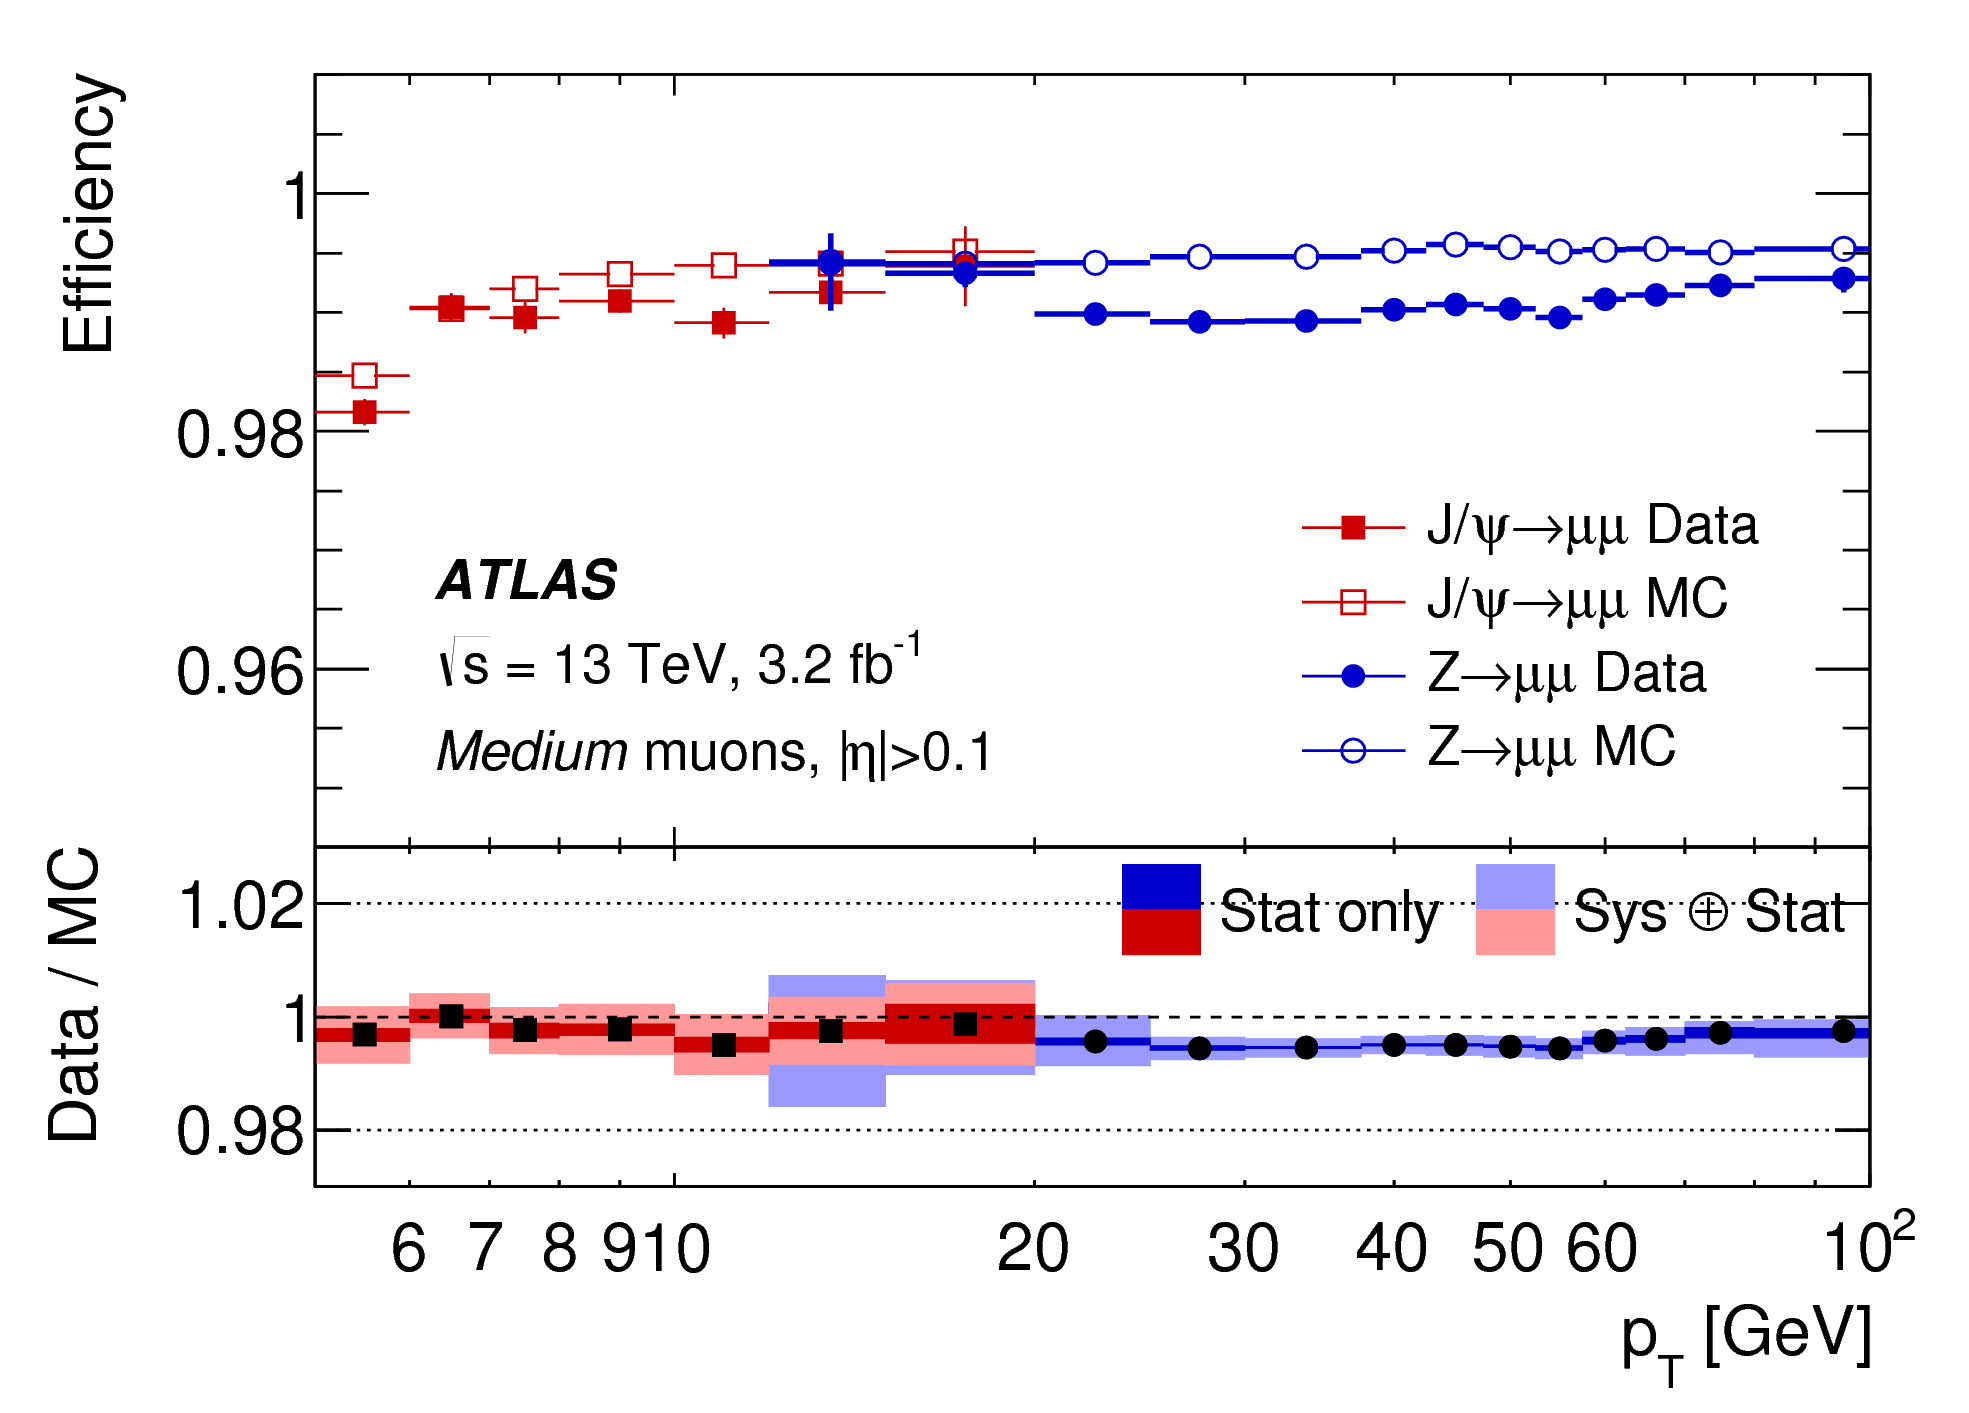
\includegraphics[width=0.9\textwidth]{figures/Objects/muoneffpt.png}
  \caption{}
  \label{sec:obj:fig:muoneffpt}
\end{subfigure}
\begin{subfigure}{0.5\textwidth}
  \centering
  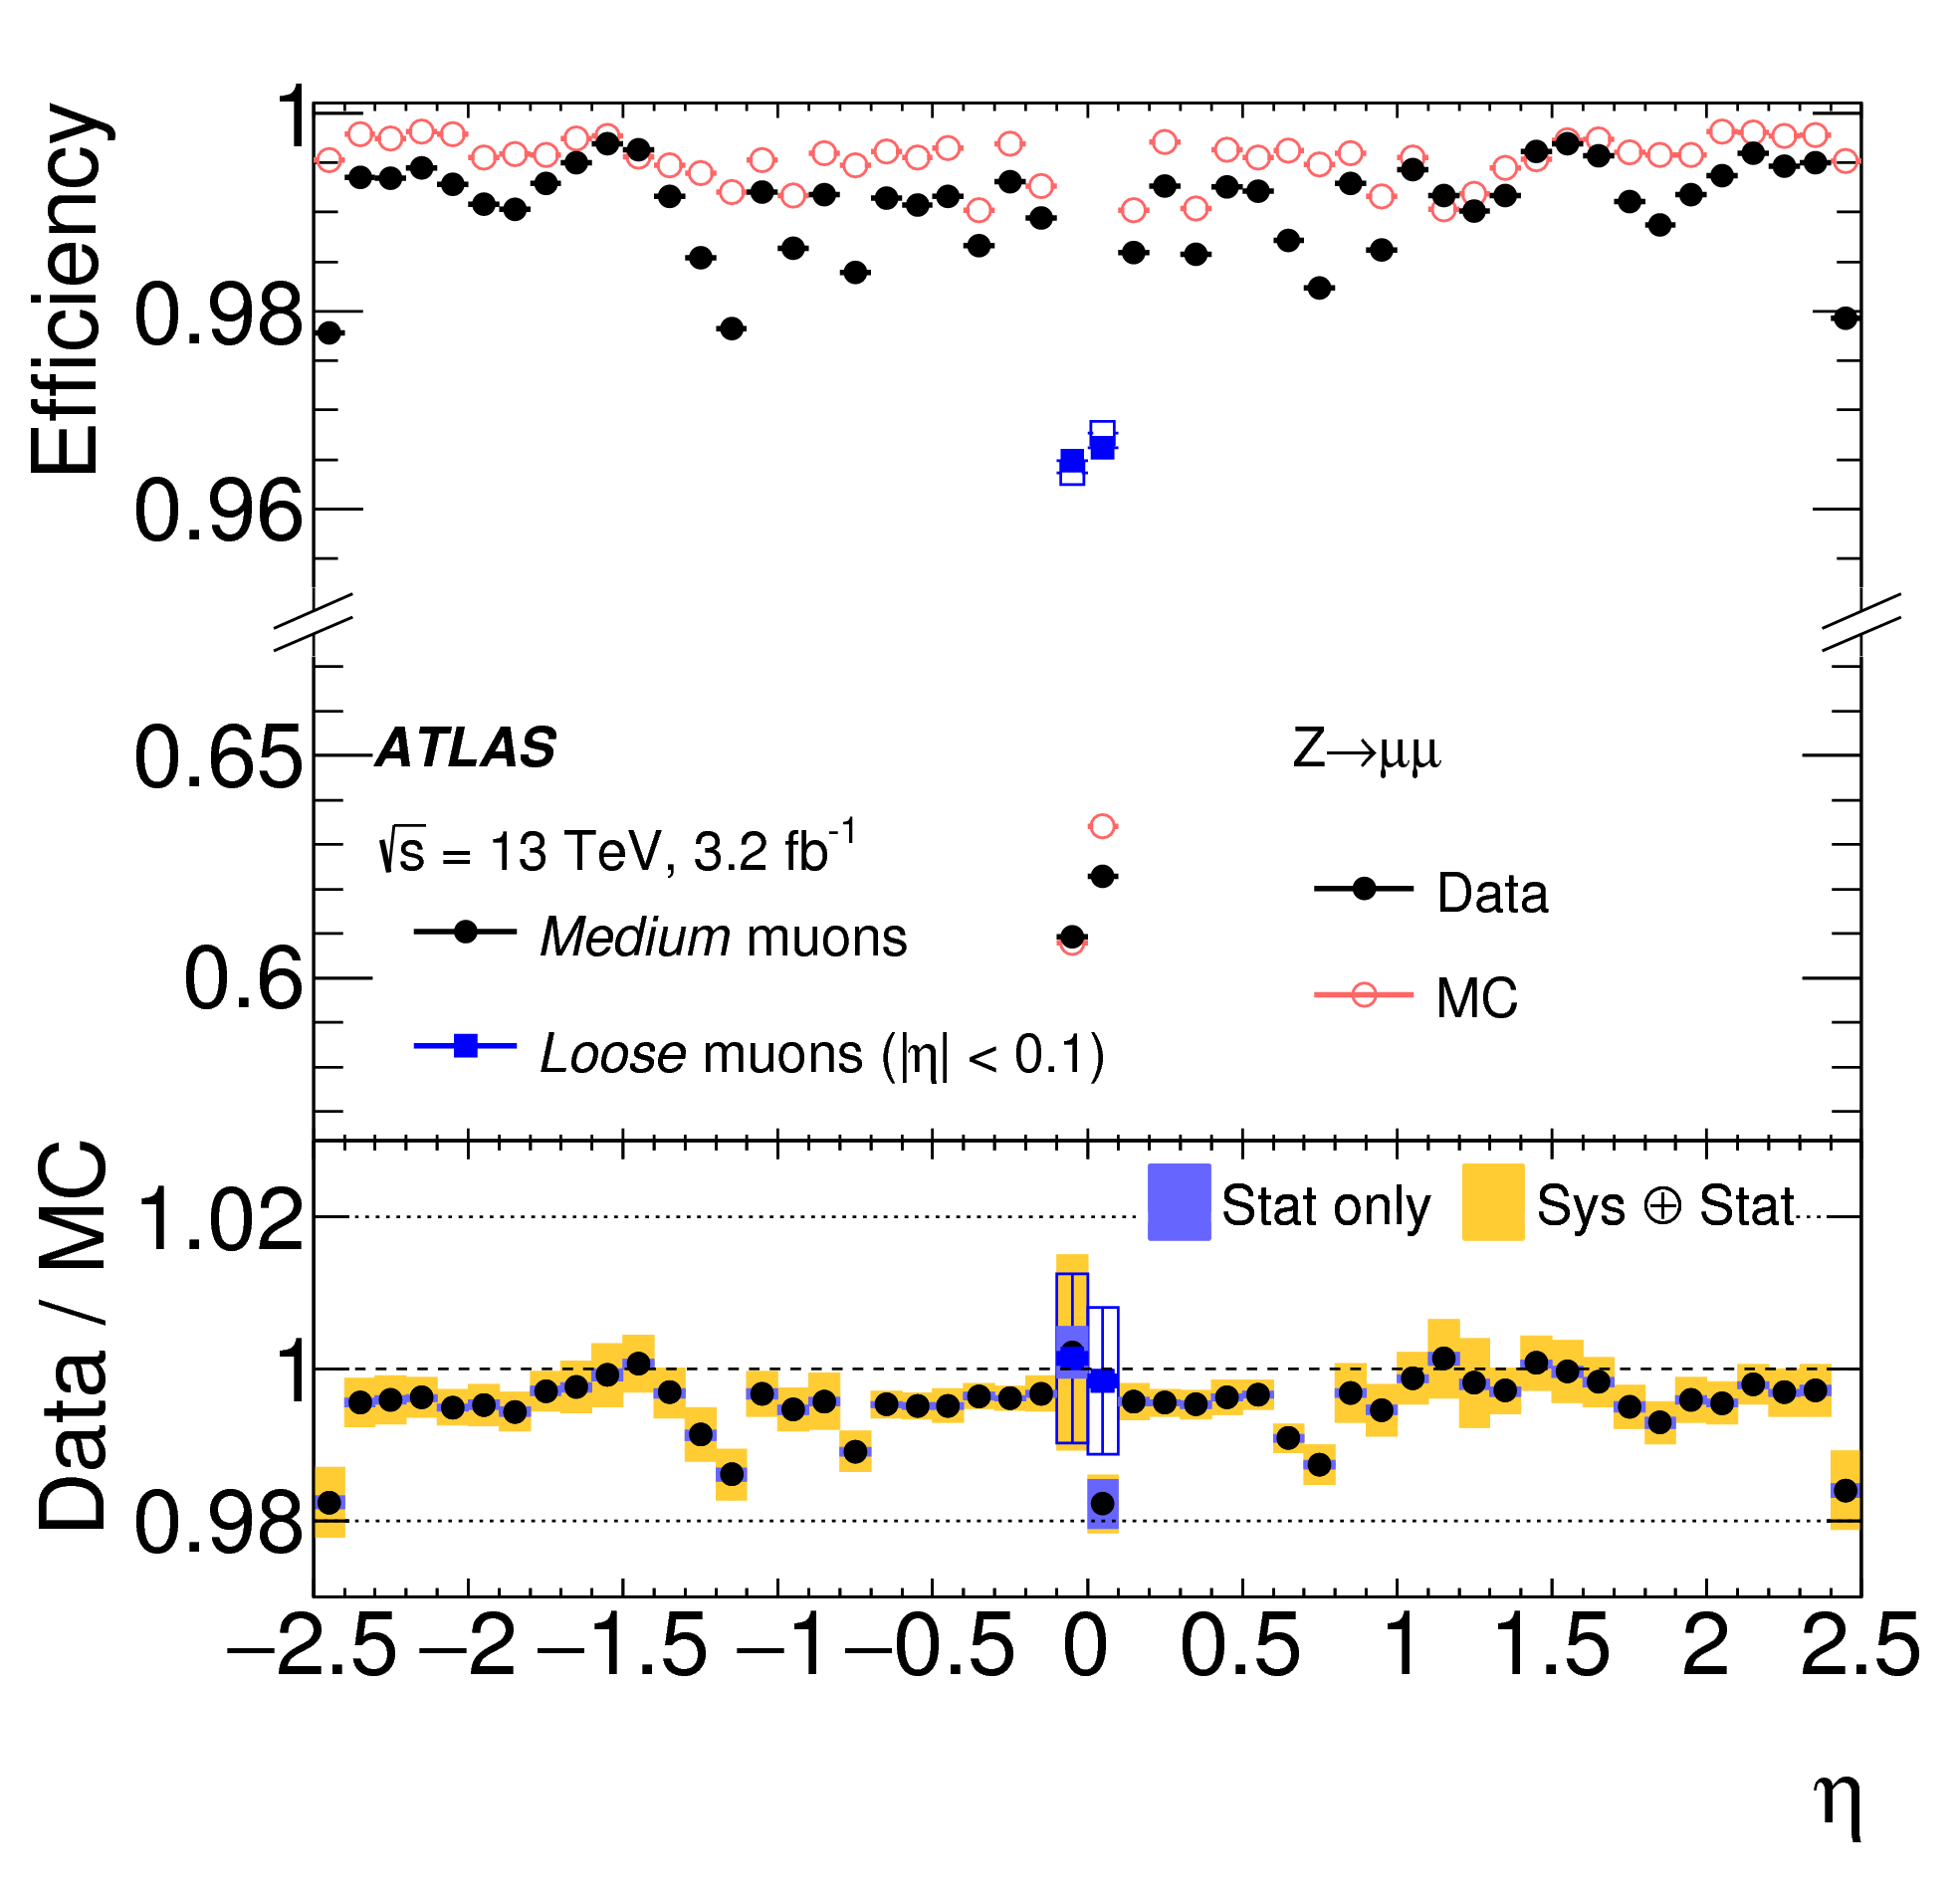
\includegraphics[width=0.675\textwidth]{figures/Objects/muoneffeta.png}
  \caption{}
  \label{sec:obj:fig:muoneffeta}
\end{subfigure}

\captionsetup{width=0.85\textwidth} \caption{\small Muon reconstruction efficiencies for the different operating points obtained using the tag-and-probe method in $Z\to \mu^{+}\mu^{-}$ and $J/\Psi \to \mu^{+}\mu{-}$ events, as a function of  (a) transverse momentum $\pt$ and (b) pseudorapidity $\eta$. From reference \cite{Aad:2016jkr}.}
\label{sec:obj:fig:muoneff}
\end{figure}

The muon momentum scale has been measured in data using $Z\to \mu^{+}\mu^{-}$ and $J/\Psi \to \mu^{+} \mu^{-}$ events. Correction factors as a function of the muon $\pt$ in different regions of $\eta$ are derived to match the known value of the $Z$-boson mass. The total uncertainty on the muon momentum scale varies from a minimum of < 0.05$\%$ in the barrel region to a maximum of 0.3$\%$ for $|\eta|\sim 2.5$ \cite{Aad:2016jkr}. The main way to probe the muon momentum resolution is provided by the study of the $Z$ and $J/\Psi$ resonance width. It is found that the resolution in data is slightly worse than that in simulation, and appropriate corrections are derived and applied to simulation to match the data.\par
As briefly discussed above, the analyses presented in this dissertation use the medium combined muons and {\sl Gradient} muon isolation is required to reject muons from semileptonic hadron decays. A different muon definition, with no isolation requirement, will also be used to estimate the contribution of multijet events as described in section \ref{chp:sec:sigbkg:qcd}.
